\section{Introduction}
\label{sec:introduction}

% state the learning objective 
In this laboratory assignment we study the purely resistive circuit 
shown in Figure~\ref{fig:circuit}.

We started with the theoretical analysis of the circuit, 
firslty using the nodal method and secondly mesh analysis. 
This procedure is explored in section ~\ref{sec:analysis};
We used the software \textit{Octave} to solve the derived systems of equations.

Following this, we simulated the circuit using the software \textit{Ngspice}. 
Subsequently we compared the results of the simulation with the theoretical
results. This is described in section ~\ref{sec:simulation}.

Finally, the conclusions of this study are indicated in
Section~\ref{sec:conclusion}.

\begin{figure}[ht] \centering
    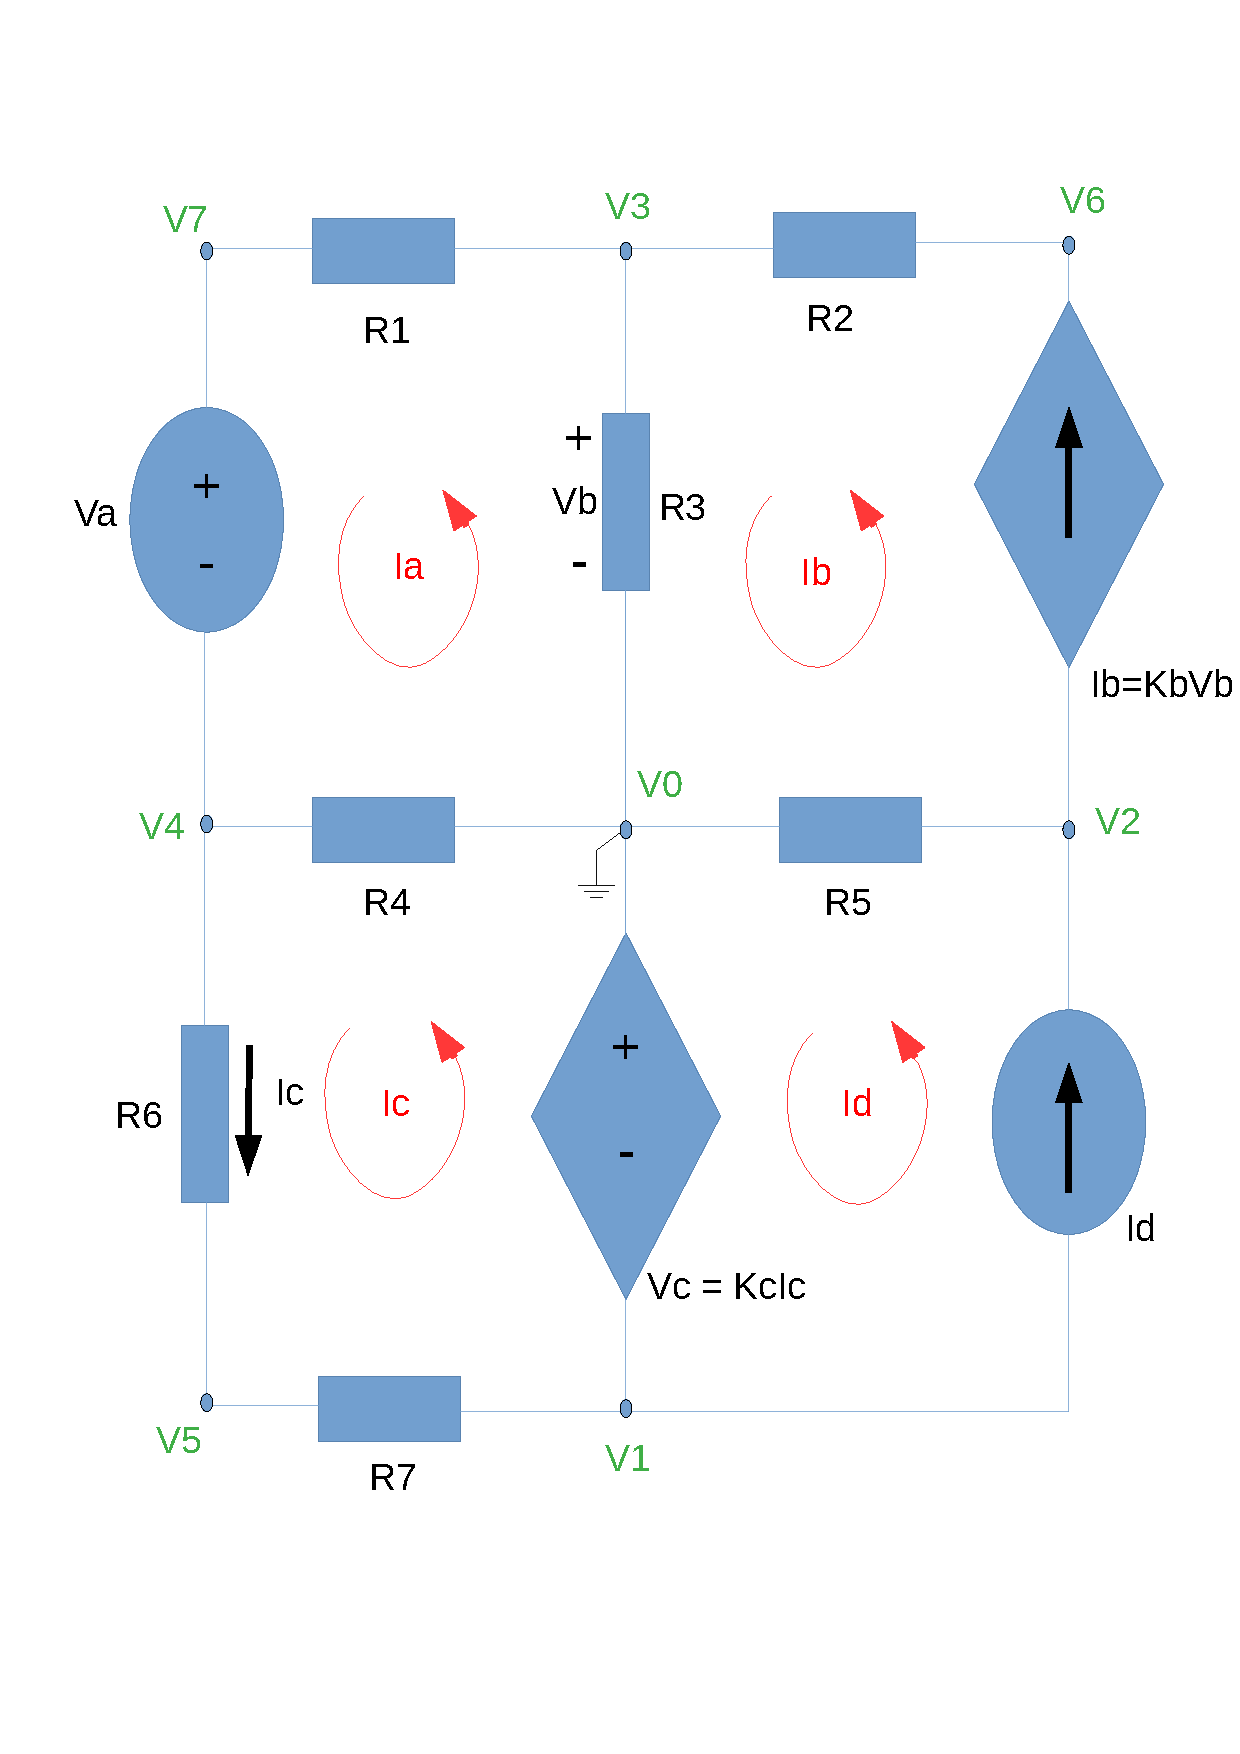
\includegraphics[width=0.4\linewidth]{circuito_tcfe.pdf}
    \caption{Circuit}
    \label{fig:circuit}
\end{figure}

